\chapter{Understanding the GPGPU}\label{chp:GPGPU}

\chapterquote{Hardware: The parts of a computer system that can be
  kicked.}{Jeff Pesis}



% Motivate the use of GPUs

Because of the evergrowing demand for new effects and more detail in
computer games and other 3D graphics applications, GPU's have seen a
massive increase in power over the last decade, as evidenced by
\reffig{fig:gflops}. A similar figure comparing the theoretical
throughput of GPU's and CPU's can be seen in \citebook{CUDAPG}. With
this in mind it is easy to understand why one would want to perform
ray tracing entirely on the GPU.

\begin{figure}
  \centering
  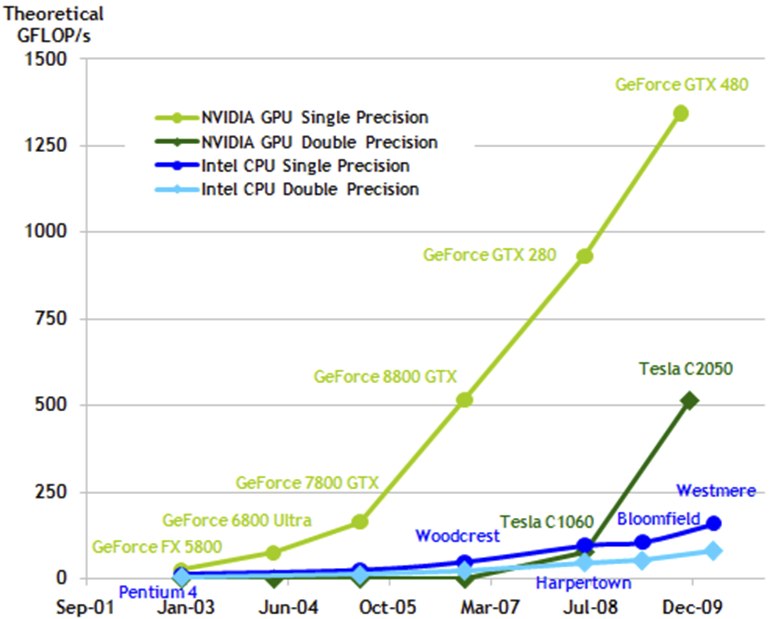
\includegraphics[width=8cm]{GFLOPS}
  \caption{A comparison of the development of floating point
    operations per second on GPU's and CPU's. \\The figure is borrowed
    from Chapter 1 in \citebook{CUDAPG}.}
  \label{fig:gflops}
\end{figure}

% What is different form CPUs

Utilizing all this power effectively, however, is not straightforward
and in order to create algorithms on the GPU that run faster than their
CPU counterparts, we need to understand how the GPU works.

The reason behind the difference in theoretical throughput seen in
\reffig{fig:gflops}, is that the CPU is designed for handling all
kinds of problems, with a large cache at it's disposal and efficient
handling of control flow. The GPU on the other hand is designed for
high throughput of small, arithmetically intense, \textit{dataparallel
  programs}\footnote{Each processor performs the same instruction
  concurrently on multiple data elements.} called \textit{kernels},
which is exactly what is required of a graphics card processing
thousands of independent vertices and performing the same shading on
hundreds of thousands of color fragments.

Since the graphics card is designed to perform vertex and fragment
processing independently of their respective neighbouring threads,
this also means that when programming the graphics card, no
assumptions can be made about which thread is where in it's
execution. This presents a problem in cases where the $n$'th thread
depends on information from all previous $n-1$ threads, fx when
splitting data or calculating the minimum or maximum values of $N$
vertices. NVIDIA's CUDA remedies this somewhat by providing
synchronization commands, but since these will only synchronize a
subset of the running threads, the overall problem remains the same.

% Why not use GPU/CPU solutions

An obvious solution is ofcourse to perform easily parallisable
operations on the graphics card and leave the rest for the
CPU. However, the following quote comes to mind:

\quotebook{
  It is important to include the overhead of transferring data to and
  from the device in determining whether operations should be
  performed on the host or on the device.
}{CUDABPG}

So once it has decided to use the graphics card, one cannot simply
transfer data back to the CPU in order to perform some operation and
then transfer it back the GPU. The overhead would in many cases be too
large to see any performance increase at all.

%% Fortunatly Sengupta et al. has come up with a solution to the
%% scattering problem, which will be discussed further in
%% \refsection{sec:GPUprims}.


% Overview of the chapter

Finding effective GPGPU solutions to the above mentioned problems is
the motivation for this chapter, which is structured as follows.
First we shall take a look at the how threads and memory is organized
on the graphics card. Understanding this will be critical in
developing GPGPU efficient solutions. Then a section will present new
GPGPU scan primitives, which will help us to perform data scattering
and reductions on dataparallel hardware. I will then be discussing a
couple interesting optimization techniques on the GPGPU, while
applying them to a reduction case study.



\section{The Architecture of the GPGPU}

To understand the architecture of the GPGPU, we must first understand the
relationship and layout of threads and then the different kinds of
memory available to threads.

\subsection{The Thread Hierarchy}

% Grid, blocks, warps and threads. We will only deal with the one
% dimensional case.

The graphics card is able to handle execution of more than a million
threads sequentially. Simply considering a graphics application
running at a 1440x900 resolution should convince anyone of this. While
above I have argued that all of these threads are executed
independently of each other, NVIDIA's CUDA architecture does place
these threads in a hierarchy, which provides programmers with some
control over thread execution.

% warps

At the lowest level threads are scheduled and executed completely
parallel in small groups called \textit{warps}\footnote{The term
  originates from weaving, the first parallel thread
  technology.\citebook{CUDAPG}}, usually with a warpsize of 32. While
threads in a warp have their own instruction counter and register
state, and therefore logically can branch independently of
neighbouring threads, a warp can only execute one specific instruction
at a time. The following example should help clarify this.

\begin{algorithmic}
  \IF{threadID < 16}
    \ASSIGN{$x$}{$threadID$}
  \ELSE
    \ASSIGN{$x$}{$32 - threadID$}
  \ENDIF
\end{algorithmic}

% It is a wide SIMD/SIMT, Single-Instruction / Multiple-Thread,
% machine. This means branching hurts. Alot!

The first 16 threads in the warp will evaluate to true and thus
perform the assignment $x \leftarrow threadID$, while the next 16
threads will evaluate to false and execute the alternate statement $x
\leftarrow 32 - threadID$. Since the warp can only perform one
distinct instruction at a time, it will have to first execute $x
\leftarrow threadID$, leaving the last 16 threads idle. It next
executes the else branch, meaning the first 16 threads are left
idling. While this example shows how branching can hurt performance,
when all threads in a warp do not take the same execution path,
knowning that all threads in the warp always are synchronized can also
be very beneficial, as will be shown in
\refsection{sec:loopUnrolling}.

% TODO explain any/all/ballot?

% blocks

Warps are then organized into 3 dimensional \textit{blocks}. Blocks
are expected to reside on the same multiprocessor, which provides them
with a limit as to how many threads they can contain. On current GPU's
the limit can be up to 1024 threads per block. Having threads executed
on the same multiprocessor comes with a few benefits. It is possible
to force synchronized execution of entire blocks at specific points in
the kernels. Threads can then cooperate through fast memory local to
the multiprocessor and use it to share data. Threads can lookup their
\textit{thread index} inside a block through the 3 dimensional
\textit{threadIdx} CUDA built-in variable. Being able to lookup a
threads id is important for working with data. In the one dimensional
case the $n$'th thread will usually process the $n$'th data
element. Without the thread index this would not be possible.

% grid

Blocks are themselves arranged into the uppermost part of the thread
hierarchy, a 2 dimensional \textit{grid}. The amount of data being
processed usually defines how large the grid will be. Just like a
thread can access it's index og id, it can also lookup it's block
index inside the grid through the built-in \textit{blockDim}. A 2
dimensional thread hierarchy can be seen on
\reffig{fig:threadLayout}. The kernels in this thesis will usually
process the data as 1D linear array, so a threads global id can be
calculated as $id \leftarrow blockDim.x * blockIdx.x + threadIdx.x$.

\begin{figure}
  \centering
  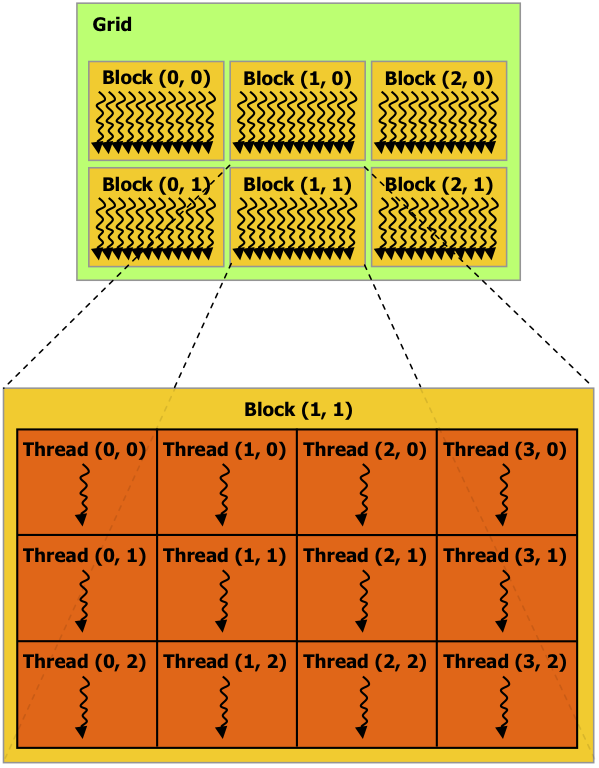
\includegraphics[width=8cm]{ThreadLayout}
  \caption{A figure of CUDA's thread hierarchy.\\ The figure is borrowed
    from Chapter 2 in \citebook{CUDAPG}.}
  \label{fig:threadLayout}
\end{figure}




\subsection{The Memory Model}

With the thread hierarchy explained, the different memory spaces made
available through CUDA can be described.  

CUDA provides the programmer with 3 overall types of memory:
\textit{global memory}, which can be accessed by any thread at any
time and persist across kernel launches, \textit{shared memory}, which
is shared across all threads in a block and persists as long as a
block is active, and finally \textit{registers}, which are local to
each thread and only exists as long as it's thread. In the following
a section is devoted to each memory space.

\subsubsection{Global Memory}

% Slow, coalescene of data types with size 1, 2, 4, 8, and 16 bytes.

Global memory, or \textit{device memory}, is the slowest form of
memory on CUDA devices. As mentioned above it persists across kernel
launches and is therefore perfect for storing input data to kernels
and their results. To avoid making lots of memory transaction to and
from global memory, a warp will try to coalesce it's threads memory
access into as few transactions as possible. How well transactions are
coalesced depends on the \textit{compute capability} of the used
graphics card, with newer graphics cards being more flexible. Suffice
it to say here that it is preferable to access memory sequantially,
ie. the $n$'th thread in a warp accesses the $n$ data element.

% Coalesced memory access, float4 instead of float3
% The alignment requirement can be forced: stuct __align__(8) {

Another restiction on coalescence is that data accessed must be of
size 1, 2, 4, 8 or 16, otherwise memory transactions will be broken up
into multiple requests. Due to this it is actually more efficient to
use the CUDA built-in struct \textit{float4} than \textit{float3}.

Requirements for coalescence on hardware of a specific compute
capability is described in Appendix G of \citebook{CUDAPG}.

% hiding latency

The scheduler can also help with hiding latency from a global memory
access. If one warp is stalled while waiting for data, another
resident warp that is ready to execute can be scheduled
instead. Utilization of the graphics hardware is therefore heavily
dependent on number of resident warps and maximizing this can be
important. Especially if memory accesses are scattered, like they will
be when ray tracing a hierarchical structure.

% Mention textures and cache. The project developed for this thesis
% will not be using textures, since global memory also has cache as of
% 2.0 hardware.

Textures also reside in device memory space. Textures are read only
but provide a fast texture cache, optimized for 2D spatial data
locality. This makes texture access faster than pure global memory
access, as a device memory read is only performed on a cache miss. On
current generation hardware, global memory can use shared memory as a
cache, so textures will not be used in this project.

\subsubsection{Shared Memory}

% Faster than global/local
% Allows threads to share data

Shared memory resides on the multiprocessors and is much faster than
global memory. It is shared by threads across their block, which
allows them to share data.

% Used to overcome the limitations of global memory.

A normal usecase for shared memory is local caching of global data
shared across multiple threads. In this case the kernel first loads
data into shared memory, then performs a block-wide synchronization if
necessary and proceeds to operate on the data in shared memory. When
the kernel has finished it's computations, the data is then dumped
back to global memory.

% Can be used as global cache on never CUDA architectures isntead of
% textures and shared mem. nice we laike

As mentioned above, on newer architecture multiprocessor memory can be
used as a cache for global memory.

% TODO? Bank conflicts, nothing is ever as good as it seems.



\subsubsection{Registers and Local Memory}

% Register

Registers are part of the threads execution context and the fastest
kind of memory on the device. Since there is only a fixed amount of
registers available per multiprocessor, a kernels register usage can
have a high impact on \textit{occupancy}\footnote{The amount of thread
  blocks resident on a multiprocessor, relative to the maximum amount
  possible.}, which in turn can have an impack on the schedulers
ability to hide latency.

% launch bounds

The compiler employs different heuristics to minimize register usage,
while keeping the kernel running efficiently. Sometimes though,
programmers may want to use even fewer registers for specific kernels,
in order to maximize occupancy and global memory latency hiding. To
this end they can aid the compilers heuristics by providing
\textit{launch bounds}. In CUDA 2 arguments can be given as launch
bounds. The first tells the compiler the maximum number of threads per
block that the kernel will ever be invoked with. The second argument
tells the compiler how many blocks should be resident on the
multiprocessor. The compiler can then use this information to derive
upper bounds for the registers per thread.

% TODO? example



% Local memory

But the compiler cannot always simply reduce the number of registers
to fit inside the launch bounds. If 20 register are needed to hold 20
distinct values, then those values have to be stored somewhere else,
if the programmer demands that only 16 registers be used. In that case
the compiler can use \textit{local memory}, which resides in device
memory and thus has the same high latency and low bandwith as global
memory. Forcing a few registers into local memory to gain occupancy
can be beneficial though, and since all threads will access local
memory at the same time, there is a high probability that local memory
access can be coalesced.

Kernel variables that the compiler will most likely place in local
memory are:

\begin{itemize}
  \item Any array that from the compilers point of view are
    dynamically indexed.
  \item Structures or arrays that are to large to fit inside registers.
  \item Any variable in the kernel, if the kernel has to many
    variables to place them all in register memory. This is referered
    to as \textit{register spilling}.
\end{itemize}



\section{The Scan Primitive}\label{sec:GPUprims}

% Scan and compact

% cite sengupta paper

\quotebook{...efficient solutions to parallel problems in which each
  output requires global knowledge of the inputs.}{Sengupta:2007}

% Useful for scattering data

% Give array example


% NVIDIA mentioned 3 optimization points

% Structures of arrays vs arrays of structs. Usefull when fx
% sorting. CUDPP article/forum. Plus cache performance.

% Unrolling loops, even when it means more work. Preprocess lower
% nodes yields nearly a 50% speedup from this.


\section{Optimization Techniques: Reduction}


\subsection{Naive implementation}


\subsection{Coalesced Memory Access}


\subsection{Switching to shared memory}

% Does that make any difference on 2.0 archs?


\subsection{Using Registers}

% Storing the thread local result in both smem and register


\subsection{Loop unrolling}\label{sec:loopUnrolling}

% Unroll the loops.

% Then move the first up to where data is loaded into shared mem

% And move the last reduction down where the final result is written.




%\section{Case Study: Segmented Reduction}

% Alot of reductions and iterative algorithms. It is therefore
% important to know how to optimize these from a naive implementation.

% Algorithm from bla

%\subsection{Naive implementation}

%\subsection{Switching to shared memory}


%\subsection{Rewriting slow math operations}

% Pow is 'expensive' and can be replaced by a simple doubling of the
% indices.

%\subsection{Unrolling the loops}

% Can be done with a template parameter. Would still need to check
% range, but could remove the loop variables. Would need a few speciel
% cases for small kernelsizes (1 - 4 threads).

% Pros

% Shared memory is almost halved

% Only needs half the threads

% No dummy variables

% Cons

% Unrolling yields more instructions for executions that would only
% loop once. However since that only account for the last couple of
% nodes, it is more than made up for by all the previous
% nodes. Version 2 could be used for executions with 2 or less threads.

% Unrolling must also adds a check for out of bounds (or replaces the
% loop with that check) However making sure that single block bounding
% box reductions are never brought to the segmented reducer will
% ensure at least 2 values exist and one bounds check can be omitted.
